% Cuboid ABCD-A1B1C1D1, AB:BB1=1:2 true ratio, cabinet depth, E midpoint of AA1.
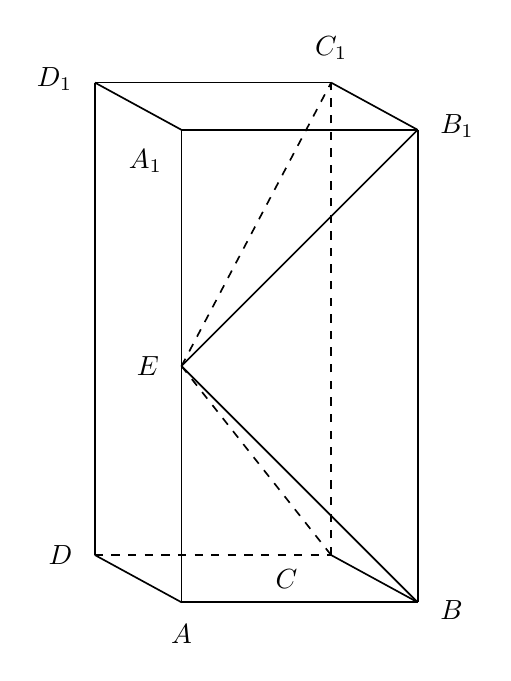
\begin{tikzpicture}[x=1mm,y=1mm,line width=.6pt,font=\normalsize]
\draw (0.0,0.0) -- (30.0,0.0);
\draw (30.0,0.0) -- (30.0,60.0);
\draw (0.0,60.0) -- (30.0,60.0);
\draw (0.0,0.0) -- (0.0,30.0);
\draw (0.0,30.0) -- (0.0,60.0);
\draw (0.0,0.0) -- (-11.0,6.0);
\draw (30.0,0.0) -- (19.0,6.0);
\draw (-11.0,6.0) -- (-11.0,66.0);
\draw (-11.0,66.0) -- (0.0,60.0);
\draw (-11.0,66.0) -- (19.0,66.0);
\draw (30.0,60.0) -- (19.0,66.0);
\draw (0.0,30.0) -- (30.0,0.0);
\draw (0.0,30.0) -- (30.0,60.0);
\draw[dashed] (-11.0,6.0) -- (19.0,6.0);
\draw[dashed] (19.0,6.0) -- (19.0,66.0);
\draw[dashed] (0.0,30.0) -- (19.0,6.0);
\draw[dashed] (0.0,30.0) -- (19.0,66.0);
\node[anchor=north east] at (-1.2,58.8) {$A_{1}$};
\node[anchor=west] at (31.6,60.5) {$B_{1}$};
\node[anchor=south] at (19.0,67.6) {$C_{1}$};
\node[anchor=east] at (-12.6,66.5) {$D_{1}$};
\node[anchor=east] at (-1.6,30.0) {$E$};
\node[anchor=north] at (0.0,-1.6) {$A$};
\node[anchor=west] at (31.6,-1.0) {$B$};
\node[anchor=east] at (16.0,3.0) {$C$};
\node[anchor=east] at (-12.6,6.0) {$D$};
\end{tikzpicture}
